% Manual_MILP_BH_cyclic_en.txt
% ver1: Nov 17, 2020

\documentclass[11pt, titlepage, dvipdfmx, twoside]{jarticle}
\linespread{1.1}

\usepackage{amsfonts}
\usepackage{amssymb}
\usepackage{amsmath}
\usepackage{amsthm}
\newtheorem{theorem}{Theorem}
\newtheorem{lemma}[theorem]{Lemma}
\usepackage{enumitem}
\usepackage{geometry}
\geometry{left=2.5cm, right=2.5cm, top=2.5cm, bottom=2.5cm}

\usepackage{mathtools}
\usepackage{comment}
\usepackage[dvipdfmx]{graphicx}
\usepackage{float}
\usepackage{framed}
\usepackage{graphicx}
\usepackage{subcaption}
\usepackage{listings}
\usepackage{color}
\usepackage{url}
 
\definecolor{codegreen}{rgb}{0, 0.6, 0}
\definecolor{codegray}{rgb}{0.5, 0.5, 0.5}
\definecolor{codepurple}{rgb}{0.58, 0, 0.82}
\definecolor{backcolour}{rgb}{0.95, 0.95, 0.92}

\newcommand{\tname}{6Hc}

%%  target name used for the example 

\newcommand{\dist}{\mathrm{dist}}
\newcommand{\target}{目標}

\newcommand{\project}{{\tt mol-infer/Cyclic}}

\title{\huge{Module 3における学習済みANNとMILP\\を使用した Branch-Heightが制限された\\ 2-Lean環式化学グラフの推定}}

\author{\project}

\begin{document}

% The following makeatletter must be after begin{document}
\makeatletter 
\let\c@lstlisting\c@figure
\makeatother


\西暦\date{\today}

\maketitle

% \cleardoublepage

\thispagestyle{empty}
\tableofcontents
\clearpage

\pagenumbering{arabic}


\section{概要}
\label{sec:Intro}

この冊子では,学習済み人工ニューラルネットワーク (ANN) の重みとバイアスと\target 値を与えられた時に,
デスクリプタ (記述子) のベクトルを推定できる混合整数線形計画法 (Mixed Integer Linear Programming; MILP) の使い方を説明する.

MILPを定義する機能はPythonで実装されていて,
COIN-ORパッケージのPuLPモデリングモジュール~\cite{PuLP1,PuLP2,PuLP3,PuLP4}を使用する.

まず,この冊子に添付されているファイルの一覧を示す.

\begin{itemize}

\item フォルダ {\tt source\_code}\\
  与えられたANNに対し,
  環式化学グラフの特徴ベクトルを推定するためのMILPを実装した
  四つのpythonスクリプトと,
  MILP定式化における各デスクリプタの最小値と最大値を含むファイルを含むフォルダ.

\begin{itemize}

\item {\tt ann\_inverter.py}\\
ANNの逆問題に対する定式化したMILPを実装したスクリプト~\cite{AN19}.

\item {\tt cyclic\_graphs\_MILP\_ec\_id.py}\\
変数を初期化し,規定のトポロジ構造~\cite{cyclic_BH_arxiv}を持つ環式化学グラフを推定するための定式化したMILPの制約を用意する関数を含むPythonスクリプト.

\item {\tt infer\_cyclic\_graphs\_ec\_id.py}\\
データを用意し,指定の入力データに対して定式化したMILPを実行するPythonスクリプト.
このスクリプトの使用に関する詳細は,第\ref{sec:Exp}節に記載されている.

\item {\tt read\_instance\_BH\_cyclic.py}\\
与えられたテキストファイルからトポロジカル仕様を読み取るために必要な関数を含むPythonスクリプト.

\item フォルダ {\tt topological\_description}\\
論文~\cite{cyclic_BH_arxiv}で詳述されている化学仕様をそれぞれ提供する六つのテキストファイルを含むフォルダ.
%
\begin{itemize}
 \item {\tt instance\_a.txt}
 \item {\tt instance\_b1.txt}
 \item {\tt instance\_b2.txt}
 \item {\tt instance\_b3.txt}
 \item {\tt instance\_b4.txt}
 \item {\tt instance\_c.txt}
 \item {\tt instance\_d.txt}
\end{itemize}

\item フォルダ {\tt ANN}\\
沸点(Bp),融点(Mp),およびオクタノール/水分配係数(Kow)
の三つの\target 特性の学習済み人工ニューラルネットワーク(ANN)に関する情報を含むフォルダ.
上記の三つの各特性${\tt property}\in \{{\tt BP, MP, KOW}\}$ について三つのファイルが提供される.
%
\begin{itemize}
\item {\tt property\_desc.csv}\\
ANNの学習で使用されるデスクリプタを含むコンマ区切り形式のファイル.

\item {\tt property\_biases.txt}\\
学習済みANNのバイアスの値を含むファイル.

\item {\tt property\_weights.txt}\\
学習済みANNの重みの値を含むファイル.
\end{itemize}
%
各ファイルのデータ形式は第\ref{sec:InOut}節で説明されており,実際の例は第\ref{sec:Exp}節で説明されてる.

% \item {\tt fv4\_cyclic\_stdout.cpp}\\
% SDF形式で保存された化学グラフの特徴ベクトルを計算するC ++プログラム.
% このプログラムの入力と出力は,MILPの解として推定されるグラフのデスクリプタ値
% を検証するためにPythonスクリプト{\tt infer\_cyclic\_graphs\_ec\_id.py}
% で動作するようにカスタマイズされている(解が存在する場合).
% このソースファイルは,{\tt fv}という名前の実行ファイルにコンパイルする必要がある.
% 
% \item {\tt fv}\\
% 上記のC ++プログラムの実行可能なバイナリファイル.
% この実行可能ファイルは,オペレーティングシステム
% Linux Mint 18.3を実行しているPC上で{\tt gcc}バージョン5.4.0によってコンパイルされている.
%
\end{itemize}
\end{itemize}



この冊子の残りの部分は,次のように構成されている.
第\ref{sec:Pre}節では使用される用語と表記法を説明する.
%
第\ref{sec:InOut}節はプログラムの入力データと出力データを説明し,
第\ref{sec:Exp}節は入力データと計算結果の具体例を示す.

% \newpage

\section{用語と表記法}
\label{sec:Pre}
%
この節では,この冊子で使用されている用語と表記法について説明する.


\begin{itemize}

\item {\bf 特徴ベクトル}\\
%
特徴ベクトルは,デスクリプタと呼ばれる特定のパラメータの数値を格納する.
本研究では,非水素原子の数,ある程度の頂点の数など,グラフ理論のデスクリプタを選択する.

\item {\bf 人工ニューラルネットワーク - ANN}\\
%
人工ニューラルネットワークは,機械学習の方法の一つである.
入力の特徴ベクトルと出力の\target データのペア間の相関関数を構築する方法を提供する.


\item {\bf 入力層, 中間層, 出力層}\\
%
順伝播型ニューラルネットワークの多層パーセプトロンモデルを扱う.
これらのニューラルネットワークは、いくつかの層で構成されている.
最初に入力層があり,各ニューロンは特徴ベクトルの一つの値を入力として受け取る.
次に隠れ層がある.ここでは,入力層からの値が順伝播的に伝播され,一つの層の各ノードが次の層の全てのノードに接続される.
最後に,出力は出力層で与えられる.
単一の\target 値の予測を扱うため,出力層は単一のノードで構成されていると仮定する.

\item {\bf 重み}\\
%
ANN内の二つのノードを接続する各辺には,重みと呼ばれる実数値が割り当てられる.
ANNの学習プロセスの一部で,既知の特徴ベクトルと\target 値のペアに基づいて,それぞれの重みの値を決定する.

\item {\bf バイアス}\\
入力層のノードを除くANNの各ノードには,バイアスと呼ばれる実数値が割り当てられる.バイアスは辺の重みと同様に,学習プロセスを通じて決定される.


\item {\bf 活性化関数}\\
%
ANNでは,各ノードは入力の活性化関数と呼ばれる関数として出力を生成する.
各ノードには,活性化関数としてRectified Linear-Unit(ReLU)関数があると仮定する.これはANNの逆問題のMILP定式化~\cite{AN19}で正確に表すことができる.
%https://scikit-learn.org/stable/modules/generated/sklearn.neural\_network.MLPRegressor.html

\item {\bf 混合整数計画問題(MILP)}\\
%
すべての制約が線形式として与えられ,
いくつかの決定変数が整数値のみを取る必要がある数理計画問題の一種.
MILPの標準的な文献として,\cite{LP}を挙げておく. 

\item {\bf グラフ}\\
頂点の有限集合とエッジの有限集合で構成される抽象的な組合せ構造.ここで各辺は頂点のペアである.
無向グラフを扱う.すなわち,辺が順序付けられていない頂点のペアになっているグラフを扱う.
グラフ理論の初等的な内容に関しては様々な文献 (たとえば~\cite{graph}など) が知られている.

\end{itemize}

% \newpage

\section{プログラムの入力と出力}
\label{sec:InOut}

この節では,プログラムの入力と出力の形式について説明する.
第\ref{sec:section3_1}節ではプログラムの入力形式の例を示し,
第\ref{sec:section3_2}節では具体的な計算例を示す.
次に,第\ref{sec:section3_3}節ではプログラムの出力形式の例を示し,
第\ref{sec:section3_4}節では具体的な計算例を示す.


\subsection{プログラムの入力}
\label{sec:section3_1}

この節では、プログラムへの入力について説明する.
最初の入力には、以下を含む三つのテキストファイルが必要となる. \\
~~~~- CSV形式のデスクリプタ名, \\
~~~~- テキスト形式の学習済みANNの重みと\\
~~~~- テキスト形式の学習済みANNのバイアス. \\

プログラム実行のコマンドラインパラメータとして用いる共通の接頭辞が {\tt TT}の場合,学習済みANNのディスクリプタ名,重み,バイアスが格納されたファイルはそれぞれ {\tt TT\_desc.csv},{\tt TT\_weights.txt}, {\tt TT\_biases.txt}というファイル名で保存されていなければならない.

%
次に,学習済みANNに基づいて化学グラフを推定するための\target 値を指定する.
その次は,\cite{cyclic_BH_arxiv}で説明されているように、テキストファイルで指定された化学仕様と、第\ref{sec:section3_4}節で説明されている出力ファイルのファイル名の接頭辞を指定する.

最後に,使用するMILPソルバープログラムを選択する.以下から選択できる. \\
~~~~- 1: CPLEX(商用MILPソルバー) \cite{cplex}. \\
ファイル{\tt infer\_acyclic\_graphs.py}のパラメータ{\tt CPLEX\_PATH}は、CPLEXプログラム実行可能ファイルの正しいパスに設定する必要があることに注意せよ.\\
~~~~- 2: CBC(無償のオープンソースMILPソルバー).Python用のPuLPパッケージ\cite{PuLP1}に付属している.




\subsection{入力データ形式}
\label{sec:section3_2}

この節では,プログラムの実際の入力例を示す.
特に,第\ref{sec:section3_1}節で述べた三つの入力ファイルの具体例を示す.

このプログラムの目的は,与えられた学習済みANNから所望の出力を生成する特徴ベクトルを計算することである.
図\ref{fig:sample}は学習済みANNの例を示す.


\begin{figure}[H]
  \centering
  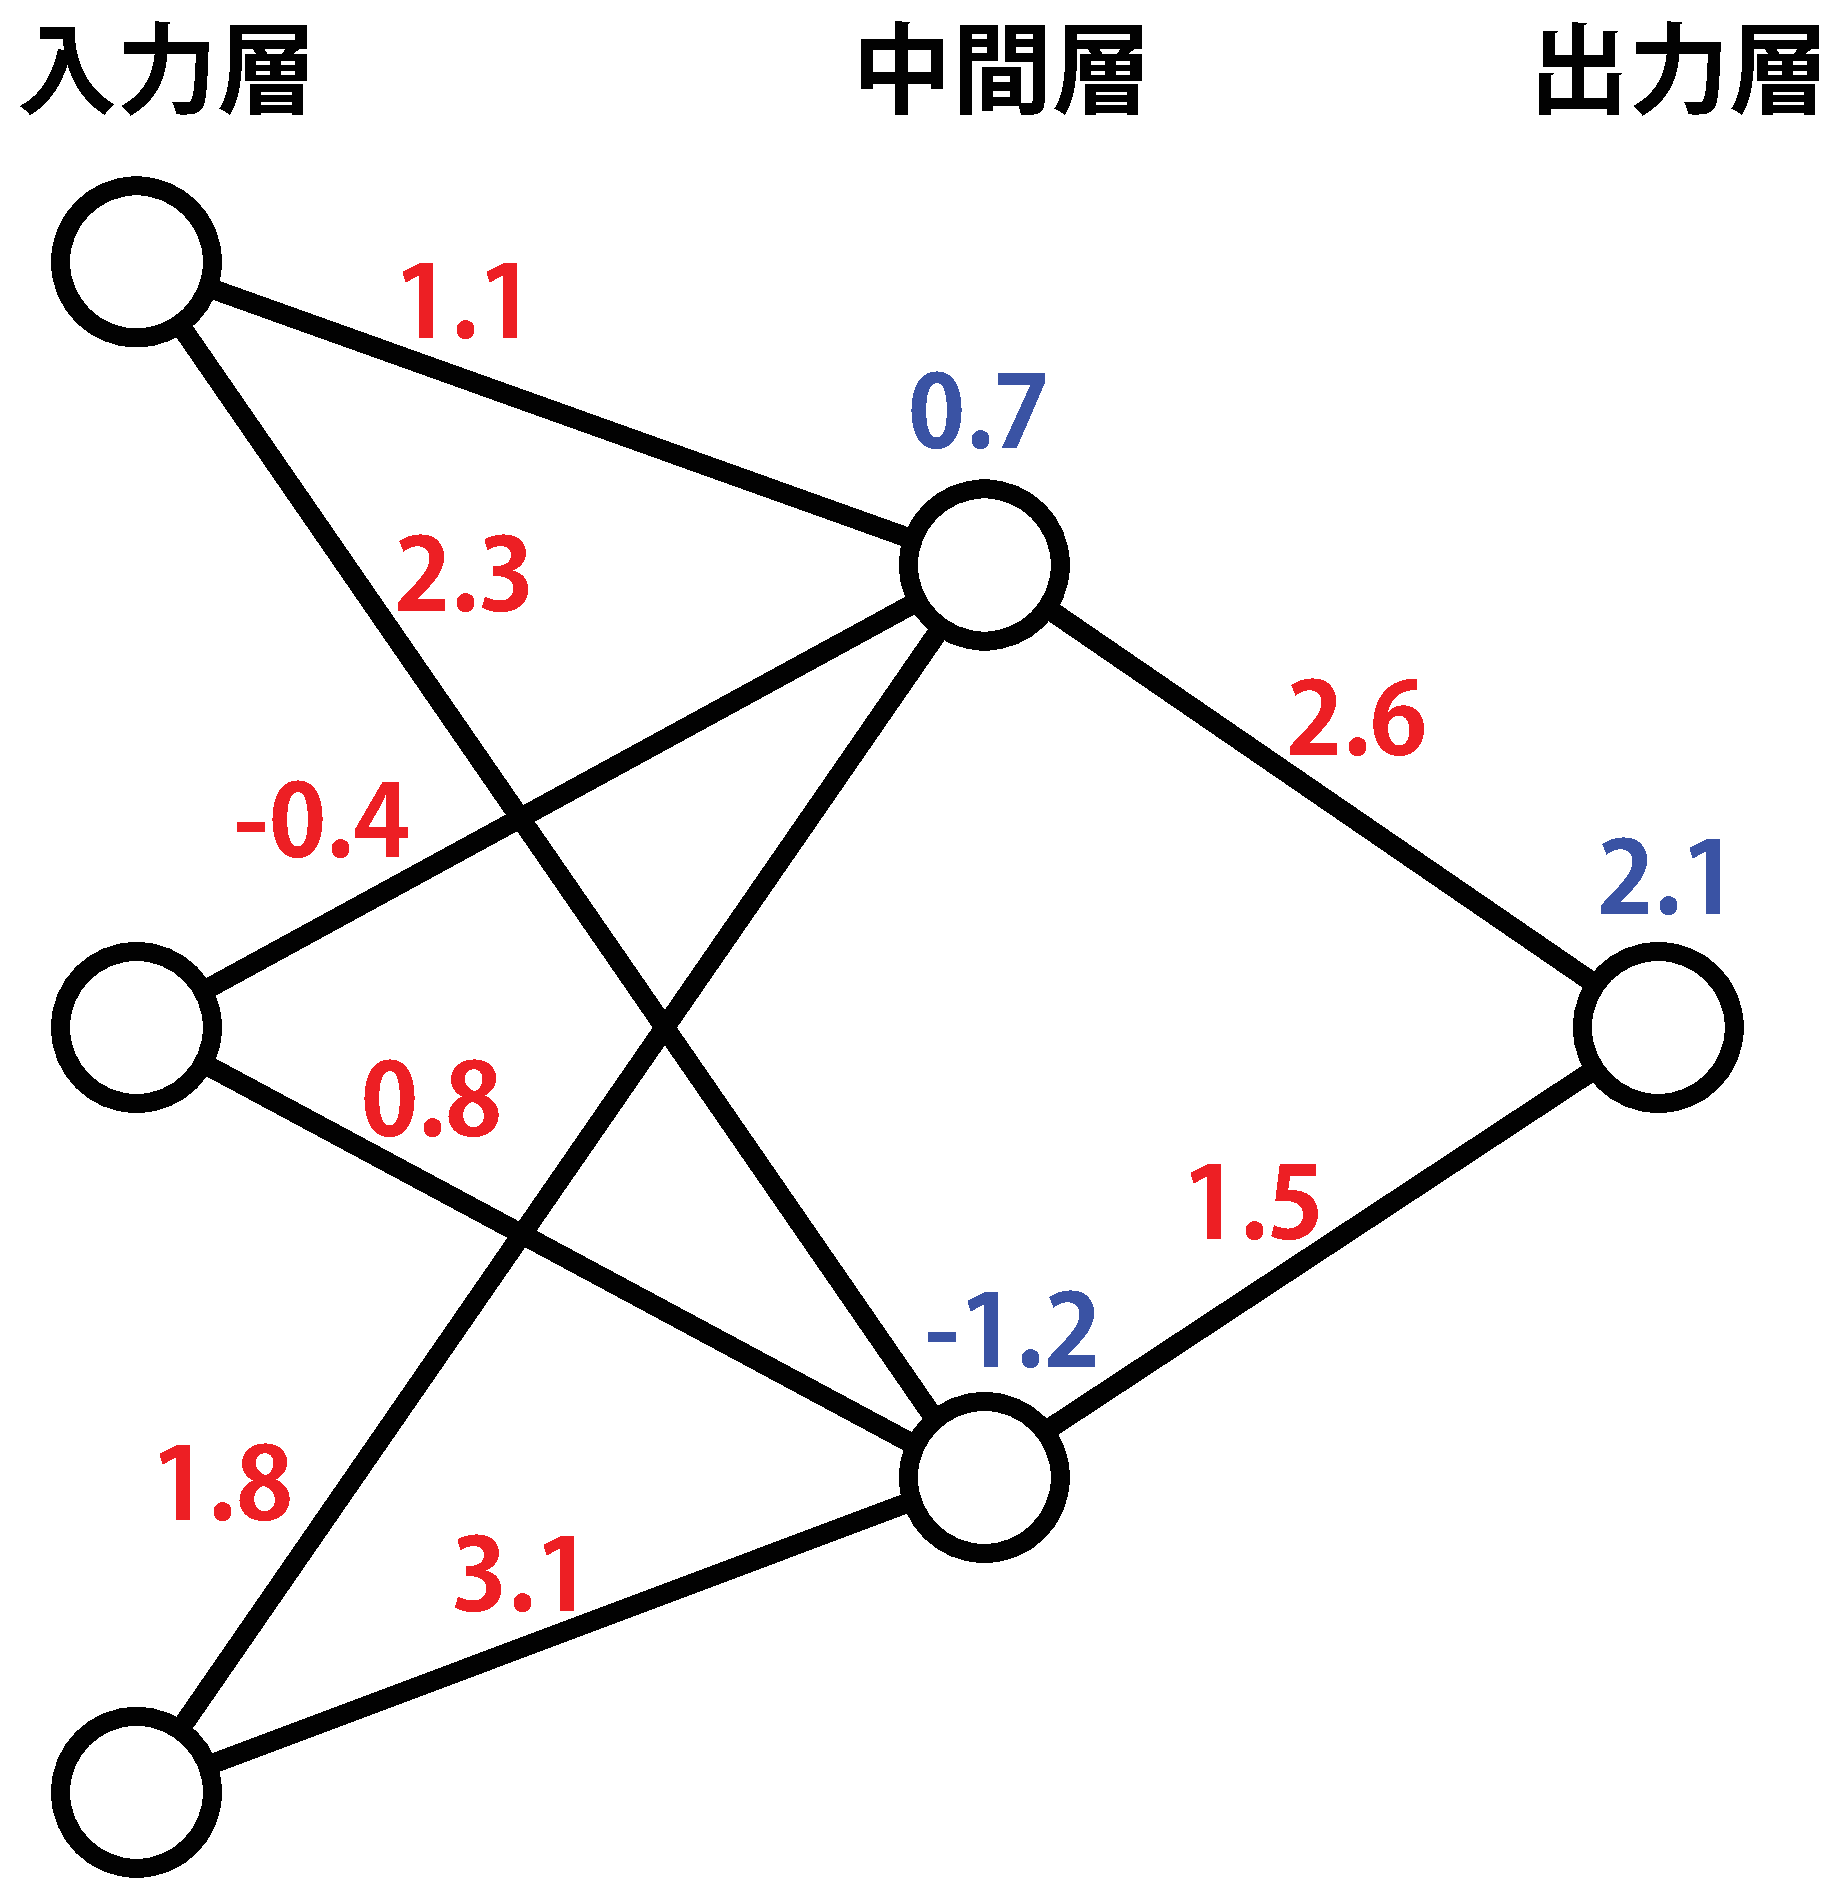
\includegraphics[width=0.5\textwidth]{./fig/ANN_sample_jp}
  \caption{学習済みANNの例.赤い数字はANNの重みを示し,青い数字はバイアスを示す.}
  \label{fig:sample}
\end{figure}


学習済みANNの重みとバイアスの情報はそれぞれ二つのテキストファイルに書き込まれる.
まず,重みの情報を含むテキストファイルの構造を示す.
このテキストファイルの最初の行には,ANNのアーキテクチャに関する情報(各レイヤーのノードの数)が書き込まれる.
2行目以降は、ANNの重みが書き込まれる.
各行は,ANNの1つのノードに接続する辺の重みが書き込まれており,最初は入力層のノードの重み,次に隠れ層のノードの重みを表している.
以下に,図\ref{fig:sample}に示されてるANNのテキストファイルの例を示す.

\bigskip

\begin{oframed}
{\bf 重みのデータ形式}\\\\
%\bigskip\bigskip
3 2 1\\
1.1 2.3\\
-0.4 0.8\\
1.8 3.1\\
2.6\\
1.5\\
\end{oframed}

\bigskip


次はANNのバイアスのテキストファイルである.
Fig.~\ref{fig:sample}のバイアスを以下に示す.

\bigskip

\begin{oframed}
{\bf バイアスのデータ形式}\\\\
%\bigskip\bigskip
0.7\\
-1.2\\
2.1\\
\end{oframed}

\bigskip

最後に, 特徴ベクトルのデータが含まれたテキストファイルの形式について説明する.
このファイルの最初の行には,特徴ベクトルで使用されるデスクリプタの名前が書き込まれている.
2行目以降は,トレーニングデータセット内の各化学グラフのデスクリプタの数値が書き込まれている.
一つの化学グラフ毎に1行書き込まれる.
例えば,{\tt ANN}フォルダの{\tt TT\_desc.csv}を確認せよ.
ここで,${\tt TT}\in \{{\tt BP, MP, KOW}\}$である.



\subsection{プログラムの出力}
\label{sec:section3_3}

この節では,プログラムの出力について説明する.
与えられた学習済みANNの予測として与えられた\target 値となるような特徴ベクトルを持つ非環式化合グラフが存在する場合,プログラムは特徴ベクトルを出力する.
そのような化学グラフが存在しない場合,存在しないと出力する.
次の節では,プログラムの出力について説明する.


\subsection{出力データ形式}
\label{sec:section3_4}

この節では,パソコン上で得られたプログラムの出力データについて説明する.
プログラムを実行すると,ターミナルに表示される標準エラーストリームにいくつかのメッセージが出力される.
MILPソルバーが計算を完了すると,計算のステータスがターミナルに表示される.

\bigskip

\begin{oframed}
{\bf ターミナル上の出力結果のデータ形式}\\\\
%\bigskip\bigskip
\begin{tabular}{l l}
 Initializing Time: 0.529                &         \# {\tt stderr}への書き込み \\
Start Solving Using CPLEX...      &       \# {\tt stderr}への書き込み \\
Status: Feasible 				&       \# 解のステータス \\
MILP y*: 223.856 				&      \# MILPで計算された\target 値  \\
ANN propagated y*: 223.856     &      \# 学習済みANNによって計算された\target 値  \\
Solving Time: 52.534                     &      \# MILPソルバーの所要時間 \\
\end{tabular}



\end{oframed}

最後に,実行可能解が存在する場合、プログラムは二つのテキストファイルを出力する.
プログラムは出力ファイルのファイル名を入力の一部として要求することに注意せよ.
出力ファイル名として与えられたパラメータが{\tt filename}であると仮定する.
結果として得られる二つのテキストファイルのファイル名を以下に示す. \\
- {\tt filename.sdf}\\
- {\tt filename\_partition.sdf}. 

\noindent
{\tt filename.sdf}は推定された化学グラフの情報がSDF(Structure Data File)形式で書き込まれている.
詳細については,公式ドキュメント(英語)を参照せよ. \\
\url{http://help.accelrysonline.com/ulm/onelab/1.0/content/ulm_pdfs/direct/reference/}\\
\phantom{\url{http://}}\url{ctfileformats2016.pdf}\\

\noindent
{\tt filename\_partition.sdf}には,\cite{cyclic_BH_arxiv}で説明されているように,{\tt filename.sdf}から非巡回部分グラフへの閉路グラフの分解が含まれている.

\section{プログラムの実行と計算例}
\label{sec:Exp}

この節では,プログラムを実行する方法と具体的な計算例について説明する.
以下は,{\tt infer\_cyclic\_graphs\_ec\_id.py}を実行する例である.

\subsection{プログラムの実行}
\label{sec:Exp_1}

まず第\ref{sec:Intro}節で説明されているように,ターミナルが{\tt source\_code}フォルダの場所に正しく移動されていることを確認する.



\noindent
{\tt 
 python  infer\_cyclic\_graphs\_ec\_id.py 
trained\_ann\_filename\_prefix
target\_value \\
 \phantom{python }
 chemical\_specification
output\_file\_name
solver\_type
 }\\

例として\target 特性の融点を使用する.ファイル名の接頭辞がMPとなる学習済みANN、\target 値を220、化学仕様のためのファイルを{\tt instance\_1.txt},MILPソルバー(パラメータ値は1)をCPLEX\cite{cplex}とする.

{\tt 
 python infer\_cyclic\_graphs\_ec\_id.py 
ANN/MP
220 \\
 \phantom{python }
chemical\_specification/instance\_a.txt
result
1
 }\\


上記のコマンドを実行すると,ターミナルプロンプトに次のテキストが表示される.

\bigskip

\begin{oframed}
{\bf ターミナル上の出力}\\\\
%\bigskip\bigskip
 Initializing Time: 0.529  \\
Start Solving Using CPLEX...\\
Status: Feasible 		\\
MILP y*: 223.856 		\\
ANN propagated y*: 223.856 \\
Solving Time: 52.534       
\end{oframed}

出力ファイル{\tt result.sdf}および{\tt result\_partition.txt}の内容を以下に示す.

\bigskip

\begin{oframed}
{\bf File {\tt result.sdf}}\\\\
\begin{verbatim}
 1
MILP_cyclic

 48 51  0  0  0  0  0  0  0  0999 V2000 
    0.0000    0.0000    0.0000 C   0  0  0  0  0  0  0  0  0  0  0  0
    0.0000    0.0000    0.0000 C   0  0  0  0  0  0  0  0  0  0  0  0
    0.0000    0.0000    0.0000 C   0  0  0  0  0  0  0  0  0  0  0  0
    0.0000    0.0000    0.0000 O   0  0  0  0  0  0  0  0  0  0  0  0
    0.0000    0.0000    0.0000 C   0  0  0  0  0  0  0  0  0  0  0  0
    0.0000    0.0000    0.0000 C   0  0  0  0  0  0  0  0  0  0  0  0
    0.0000    0.0000    0.0000 C   0  0  0  0  0  0  0  0  0  0  0  0
    0.0000    0.0000    0.0000 O   0  0  0  0  0  0  0  0  0  0  0  0
    0.0000    0.0000    0.0000 C   0  0  0  0  0  0  0  0  0  0  0  0
    0.0000    0.0000    0.0000 C   0  0  0  0  0  0  0  0  0  0  0  0
    0.0000    0.0000    0.0000 C   0  0  0  0  0  0  0  0  0  0  0  0
    0.0000    0.0000    0.0000 C   0  0  0  0  0  0  0  0  0  0  0  0
    0.0000    0.0000    0.0000 N   0  0  0  0  0  0  0  0  0  0  0  0
    0.0000    0.0000    0.0000 C   0  0  0  0  0  0  0  0  0  0  0  0
    0.0000    0.0000    0.0000 C   0  0  0  0  0  0  0  0  0  0  0  0
    0.0000    0.0000    0.0000 O   0  0  0  0  0  0  0  0  0  0  0  0
    0.0000    0.0000    0.0000 C   0  0  0  0  0  0  0  0  0  0  0  0
    0.0000    0.0000    0.0000 N   0  0  0  0  0  0  0  0  0  0  0  0
    0.0000    0.0000    0.0000 C   0  0  0  0  0  0  0  0  0  0  0  0
    0.0000    0.0000    0.0000 C   0  0  0  0  0  0  0  0  0  0  0  0
    0.0000    0.0000    0.0000 C   0  0  0  0  0  0  0  0  0  0  0  0
    0.0000    0.0000    0.0000 C   0  0  0  0  0  0  0  0  0  0  0  0
    0.0000    0.0000    0.0000 C   0  0  0  0  0  0  0  0  0  0  0  0
    0.0000    0.0000    0.0000 C   0  0  0  0  0  0  0  0  0  0  0  0
    0.0000    0.0000    0.0000 N   0  0  0  0  0  0  0  0  0  0  0  0
    0.0000    0.0000    0.0000 C   0  0  0  0  0  0  0  0  0  0  0  0
    0.0000    0.0000    0.0000 C   0  0  0  0  0  0  0  0  0  0  0  0
    0.0000    0.0000    0.0000 C   0  0  0  0  0  0  0  0  0  0  0  0
    0.0000    0.0000    0.0000 C   0  0  0  0  0  0  0  0  0  0  0  0
    0.0000    0.0000    0.0000 N   0  0  0  0  0  0  0  0  0  0  0  0
    0.0000    0.0000    0.0000 C   0  0  0  0  0  0  0  0  0  0  0  0
    0.0000    0.0000    0.0000 O   0  0  0  0  0  0  0  0  0  0  0  0
    0.0000    0.0000    0.0000 C   0  0  0  0  0  0  0  0  0  0  0  0
    0.0000    0.0000    0.0000 C   0  0  0  0  0  0  0  0  0  0  0  0
    0.0000    0.0000    0.0000 O   0  0  0  0  0  0  0  0  0  0  0  0
    0.0000    0.0000    0.0000 C   0  0  0  0  0  0  0  0  0  0  0  0
    0.0000    0.0000    0.0000 C   0  0  0  0  0  0  0  0  0  0  0  0
    0.0000    0.0000    0.0000 C   0  0  0  0  0  0  0  0  0  0  0  0
    0.0000    0.0000    0.0000 O   0  0  0  0  0  0  0  0  0  0  0  0
    0.0000    0.0000    0.0000 C   0  0  0  0  0  0  0  0  0  0  0  0
    0.0000    0.0000    0.0000 C   0  0  0  0  0  0  0  0  0  0  0  0
    0.0000    0.0000    0.0000 C   0  0  0  0  0  0  0  0  0  0  0  0
    0.0000    0.0000    0.0000 O   0  0  0  0  0  0  0  0  0  0  0  0
    0.0000    0.0000    0.0000 C   0  0  0  0  0  0  0  0  0  0  0  0
    0.0000    0.0000    0.0000 C   0  0  0  0  0  0  0  0  0  0  0  0
    0.0000    0.0000    0.0000 O   0  0  0  0  0  0  0  0  0  0  0  0
    0.0000    0.0000    0.0000 C   0  0  0  0  0  0  0  0  0  0  0  0
    0.0000    0.0000    0.0000 C   0  0  0  0  0  0  0  0  0  0  0  0
  1  2  1  0  0  0  0
  1 28  1  0  0  0  0
  1 29  1  0  0  0  0
  2  3  1  0  0  0  0
  2  4  2  0  0  0  0
  5  6  1  0  0  0  0
  5 28  1  0  0  0  0
  5 43  1  0  0  0  0
  6 29  2  0  0  0  0
  7  8  1  0  0  0  0
  7 27  1  0  0  0  0
  7 38  1  0  0  0  0
  8  9  1  0  0  0  0
  9 10  1  0  0  0  0
  9 31  1  0  0  0  0
 10 28  2  0  0  0  0
 11 21  1  0  0  0  0
 11 24  1  0  0  0  0
 12 13  1  0  0  0  0
 12 14  2  0  0  0  0
 12 18  1  0  0  0  0
 14 15  1  0  0  0  0
 15 16  2  0  0  0  0
 15 20  1  0  0  0  0
 17 18  1  0  0  0  0
 17 19  1  0  0  0  0
 19 20  1  0  0  0  0
 20 21  1  0  0  0  0
 21 23  1  0  0  0  0
 22 23  1  0  0  0  0
 22 25  1  0  0  0  0
 22 46  1  0  0  0  0
 23 24  2  0  0  0  0
 24 26  1  0  0  0  0
 25 27  1  0  0  0  0
 26 27  1  0  0  0  0
 29 30  1  0  0  0  0
 31 32  2  0  0  0  0
 31 33  1  0  0  0  0
 33 34  1  0  0  0  0
 33 35  1  0  0  0  0
 35 36  1  0  0  0  0
 36 37  3  0  0  0  0
 38 39  1  0  0  0  0
 39 40  1  0  0  0  0
 40 41  1  0  0  0  0
 40 42  1  0  0  0  0
 43 44  1  0  0  0  0
 44 45  3  0  0  0  0
 46 47  1  0  0  0  0
 47 48  3  0  0  0  0
M  END
$$$$
\end{verbatim}
\end{oframed}

\bigskip

\begin{oframed}
{\bf File {\tt result\_partition.sdf}}\\\\
\begin{verbatim}
12
18
0 1
19
0 0
20
0 0
21
0 0
22
1 3
23
0 0
24
0 1
25
0 1
26
0 0
27
0 1
28
0 2
29
0 4
15
18 12 14 15 20
1 3
18 17 19
0 3
19 20
0 0
20 21
0 0
21 11 24
0 1
21 23
0 0
22 23
0 0
22 25
0 0
23 24
0 0
24 26
0 0
25 27
0 0
26 27
0 0
27 7 8 9 10 28
4 6
28 1 29
0 2
28 5 6 29
3 5
\end{verbatim}
\end{oframed}


\begin{thebibliography}{99}
  \bibitem{AN19}
    T.~Akutsu and H.~Nagamochi.
    A Mixed Integer Linear Programming Formulation to Artificial Neural Networks,
    in Proceedings of the 2019 2nd International Conference on Information Science and Systems,
    pp.~215--220, https://doi.org/10.1145/3322645.3322683.
    
  \bibitem{cyclic_BH_arxiv}
	  T.~Akutsu and H.~Nagamochi.
	  A Novel Method for Inference of Chemical Compounds with Prescribed Topological Substructures Based on Integer Programming.
	  Arxiv preprint, arXiv:2010.09203
	  
%   \bibitem{graph}茨木俊秀,永持仁,石井利昌.グラフ理論ー連結構造とその応用ー.朝倉書店,2010. 
%   
%   \bibitem{LP}福島雅夫.数理計画入門.朝倉書店,2012. 
  \bibitem{LP}J.~Matousek and B.~G\"{a}rtner.
			      Understanding and Using Linear Programming. Springer, 2007.
			      
  \bibitem{graph}M.~S.~Rahman.
			      Basic Graph Theory. Springer, 2017.
  
  \bibitem{PuLP1}A Python Linear Programming API, \url{https://github.com/coin-or/pulp}.
  
  \bibitem{PuLP2}Optimization with PuLP, \url{http://coin-or.github.io/pulp/}.
  
  \bibitem{PuLP3}The Python Papers Monograph, \url{https://ojs.pythonpapers.org/index.php/tppm/article/view/111}.
  
  \bibitem{PuLP4}Optimization with PuLP, \url{https://pythonhosted.org/PuLP/}.
  
  \bibitem{cplex}
{IBM ILOG CPLEX Optimization Studio~12.8 User Manual}.
\newblock
  \url|https://www.ibm.com/support/knowledgecenter/SSSA5P_12.8.0/ilog.odms.studio.help/pdf/usrcplex.pdf|.
  
\end{thebibliography}

\end{document}
